% One out-of-core spill segment = a triple of files sharing a stem. The .act mmap
% maps each address key to a u64 slot; the slot indexes the length-framed .vals
% sidecar; the .paths file is the value-less structural manifest.
\documentclass[border=8pt]{standalone}
\usepackage{tikz}
\usepackage{xcolor}
\usetikzlibrary{arrows.meta}
\definecolor{actc}{HTML}{4F46E5}
\definecolor{valc}{HTML}{0D9488}
\definecolor{pathc}{HTML}{475569}
\definecolor{magicc}{HTML}{DC2626}
\begin{document}
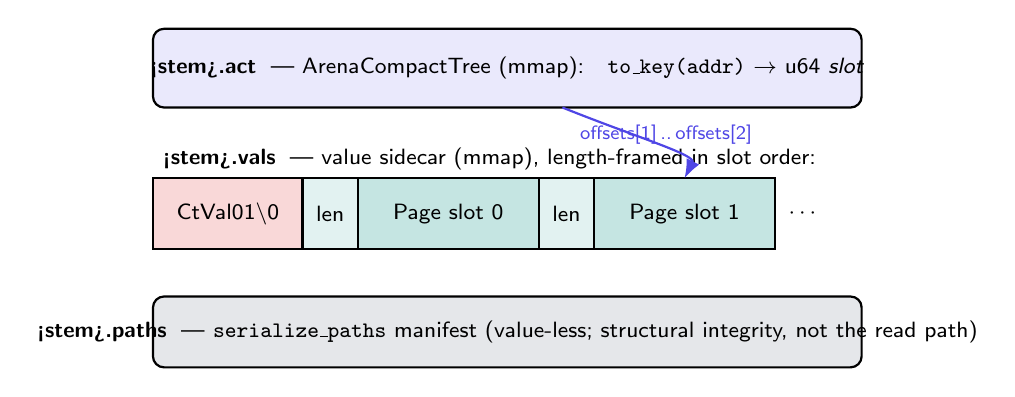
\begin{tikzpicture}[font=\sffamily\footnotesize, x=1cm, y=1cm]
  % .act
  \draw[thick, fill=actc!12, rounded corners] (0,4.1) rectangle (9,5.1);
  \node[align=left] at (4.5,4.6) {\textbf{<stem>.act} \;— ArenaCompactTree (mmap):\;\; \texttt{to\_key(addr)} $\rightarrow$ u64 \emph{slot}};

  % .vals row label
  \node[anchor=west] at (0,3.45) {\textbf{<stem>.vals} \;— value sidecar (mmap), length-framed in slot order:};
  % .vals byte frames
  \draw[thick, fill=magicc!18] (0,2.3) rectangle (1.9,3.2); \node at (0.95,2.75) {CtVal01\textbackslash0};
  \draw[thick, fill=valc!12] (1.9,2.3) rectangle (2.6,3.2); \node at (2.25,2.75) {len};
  \draw[thick, fill=valc!24] (2.6,2.3) rectangle (4.9,3.2); \node at (3.75,2.75) {Page slot 0};
  \draw[thick, fill=valc!12] (4.9,2.3) rectangle (5.6,3.2); \node at (5.25,2.75) {len};
  \draw[thick, fill=valc!24] (5.6,2.3) rectangle (7.9,3.2); \node at (6.75,2.75) {Page slot 1};
  \node[anchor=west] at (7.95,2.75) {$\cdots$};

  % slot arrow from .act into the slot-1 frame
  \draw[-{Latex[length=2.4mm]}, thick, actc] (5.2,4.1) .. controls (6.2,3.7) and (6.9,3.5) .. (6.75,3.2);
  \node[anchor=west, actc, font=\sffamily\scriptsize] at (5.3,3.75) {offsets[1]\,..\,offsets[2]};

  % .paths
  \draw[thick, fill=pathc!14, rounded corners] (0,0.8) rectangle (9,1.7);
  \node[align=left] at (4.5,1.25) {\textbf{<stem>.paths} \;— \texttt{serialize\_paths} manifest (value-less; structural integrity, not the read path)};
\end{tikzpicture}
\end{document}
